\chapter{Experimentelle Modalanalyse des Modellflugzeugs}
\label{sec: Hauptkapitel 1}

\section{Aufgabenstellung}
    % Grundsätzliches Ziel
    %---------------------
    Bei dieser Laboraufgabe sollen die tieffrequenten Schwingungsmoden des
    Modellflugzeugs bestimmt werden. Die Bestimmung der Moden soll mittels
    experimenteller Modalanalyse durchgeführt werden.
    \\
    %----------------------------------------------------------------------------

    % Ausdetaillierung
    %-----------------
    \noindent
    Es soll dabei bei der Bestimmung der Übertragungsfunktionen kein fertiger
    FRF-Block von Labview verwendet werden. Stattdessen sollen die
    Übertragungsfunktionen durch Division des gemessenen Ausgangs- durch
    Eingangssignals bestimmt werden.
%================================================================================

\section{Versuchsaufbau}
    % Diskretisierung des Fliegers
    %-----------------------------
    Da die Messung nur an jeweils einzelnen Punkten durchgeführt werden kann,
    wird in einem ersten Schritt der Modllflieger diskretisiert. Die Messpunkte
    werden dabei mittels Klebenband gekennzeichnet und über Nummern
    unterschieden. Bei der Diskretisierung wird das Modellflugzeug in 3 Bereiche
    unterteilt.
    %----------------------------------------------------------------------------

    % Tab. - Diskretisierung
    %-----------------------
    \begin{table}[h]
        \centering
        \begin{tabular}{|p{3.5cm}|p{3cm}|p{5cm}|}
            \hline
            \textbf{Bereich} &   \textbf{Schriftfarbe}    &   \textbf{Anzahl der Messpunkte}   \\
            \hline \hline
            vorderer Tragflügel &   rot &   5   \\
            \hline
            Rumpf   &   grün    &   3   \\
            \hline
            hintere Flosse  &   blau    &   2   \\
            \hline
        \end{tabular}
        \label{tab: Fliegerdiskretisierung}
    \end{table}
    %----------------------------------------------------------------------------

    \noindent
    Das diskretisierte Modellflugzeug ist in Abbildung
    \ref{fig: Flieger_diskretisiert} zu sehen.

    % Bild - Diskretisiertes Modellflugzeug
    %--------------------------------------
    \begin{figure}[H]
        \centering
        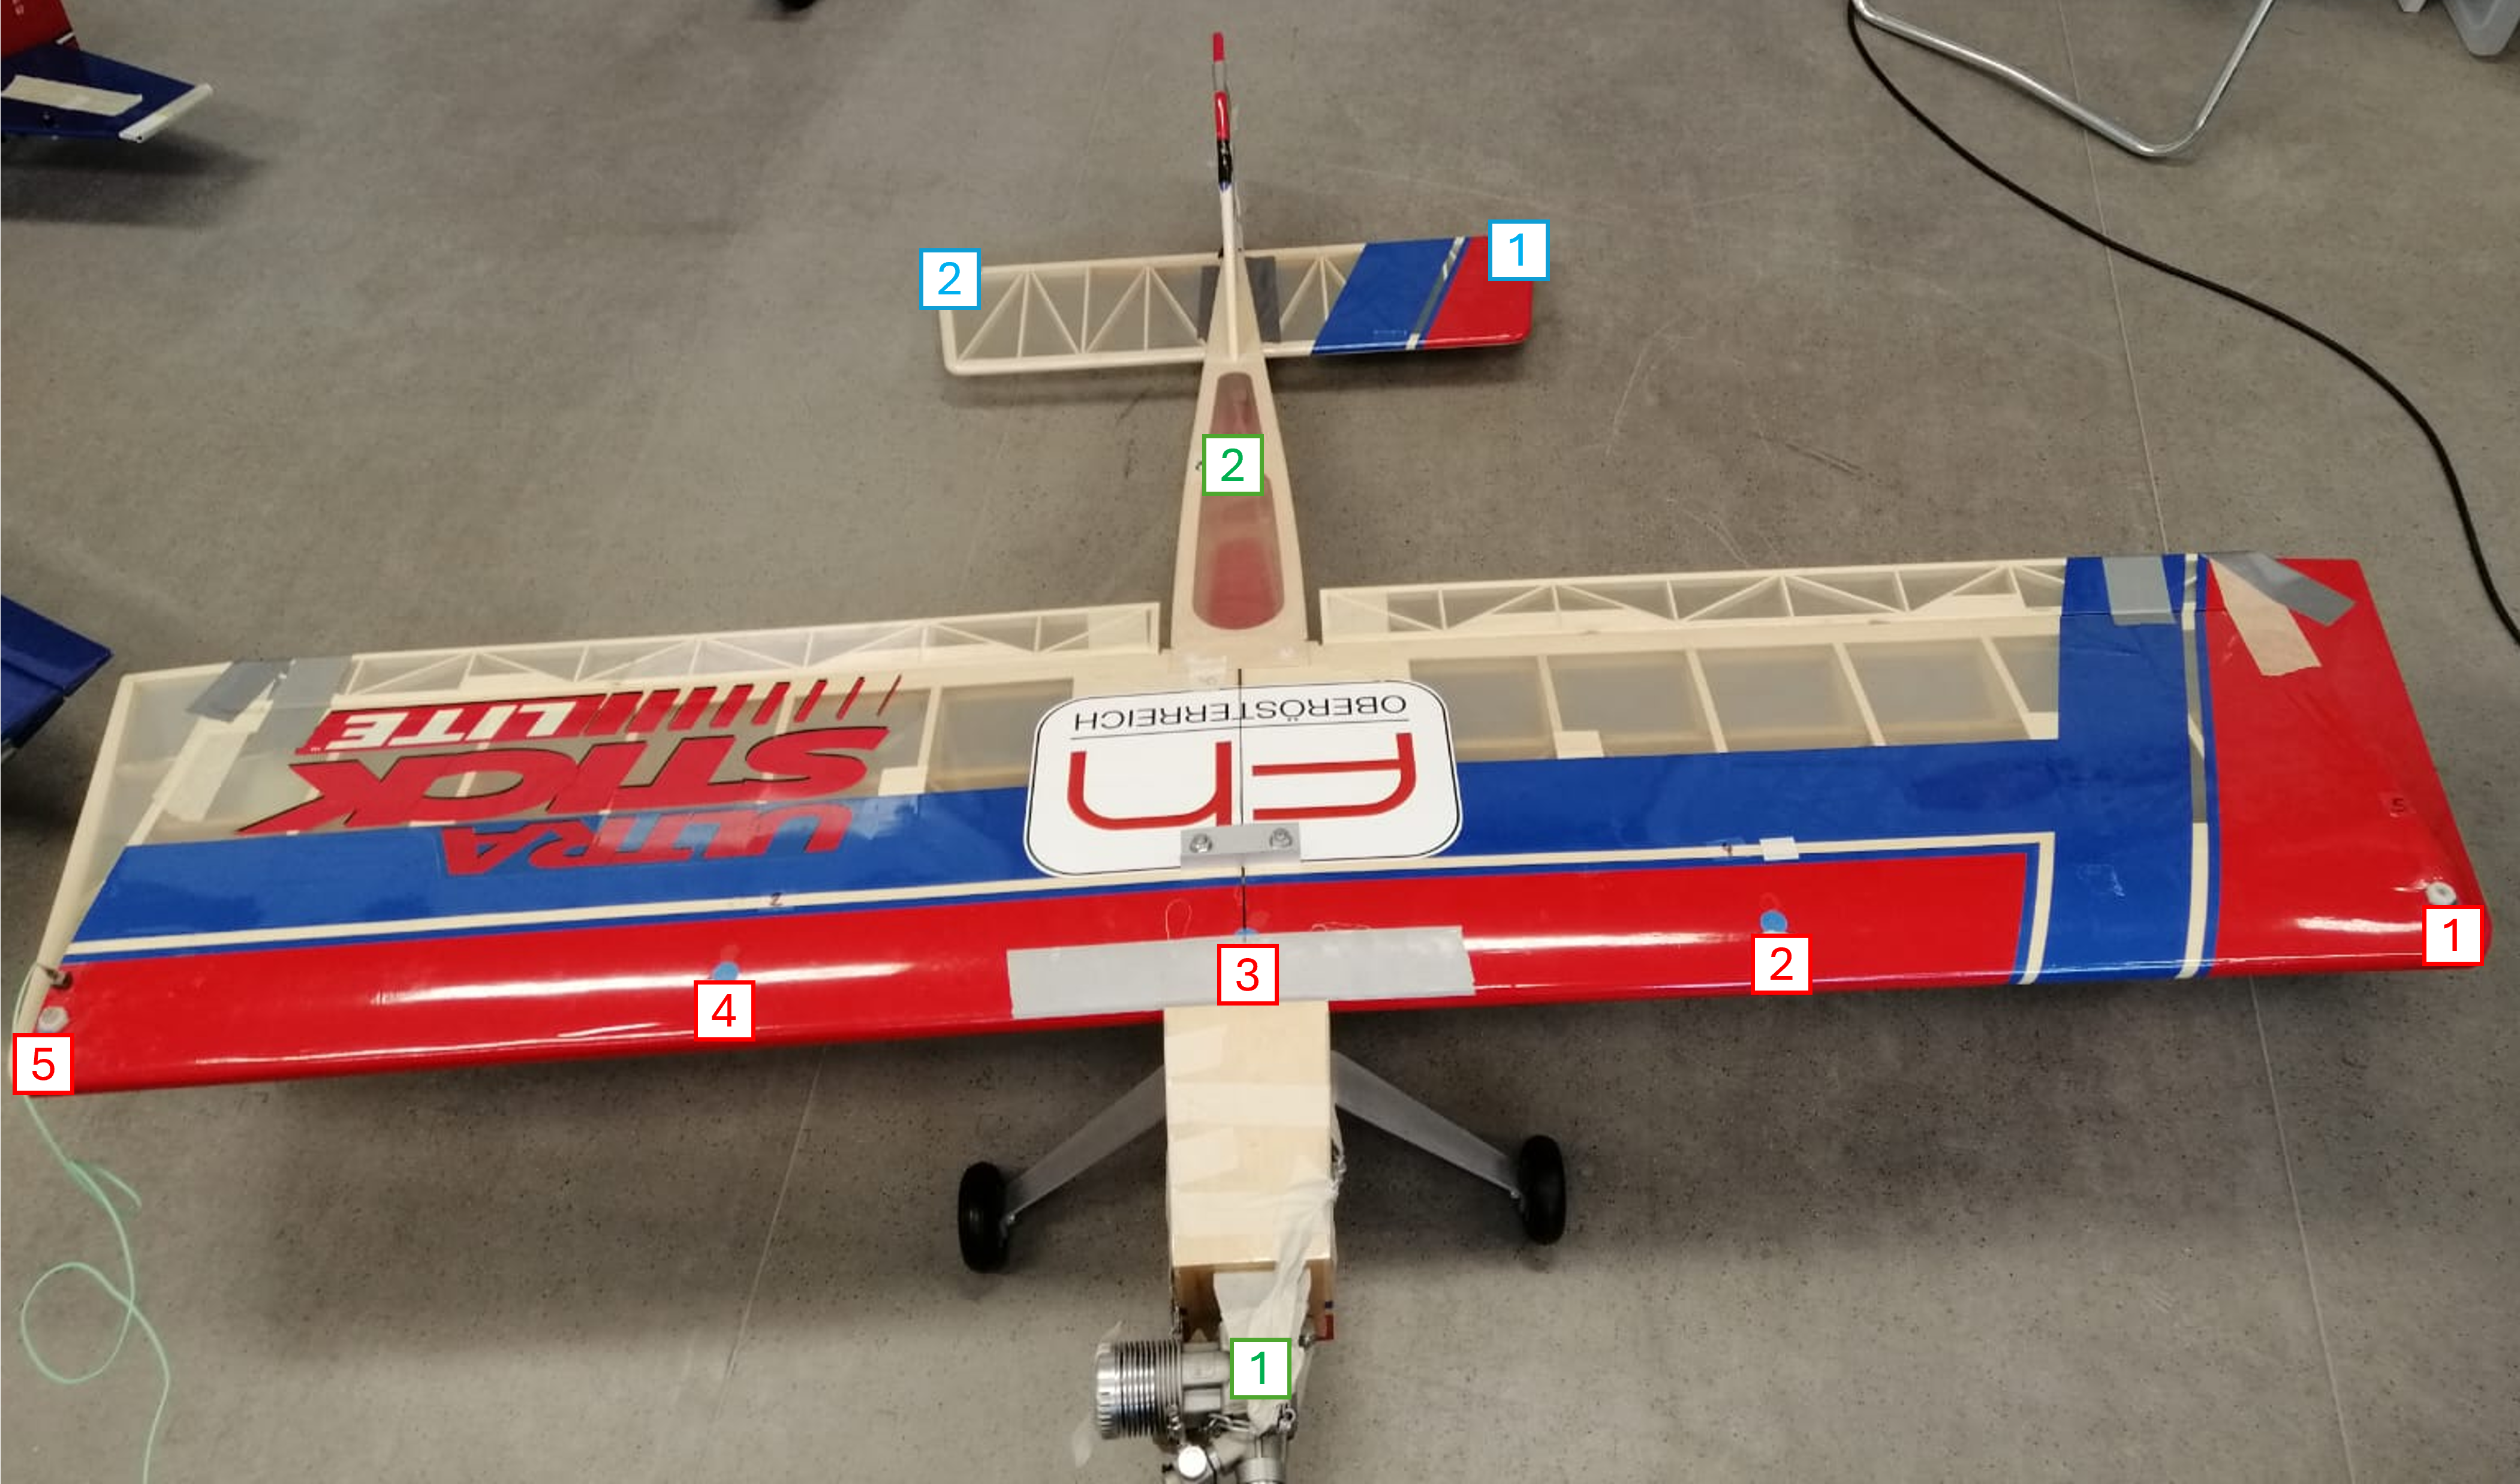
\includegraphics[width=0.95\textwidth]{Flieger_diskretisiert_Comp.png}
        \caption{diskretisiertes Modellflugzeug}
        \label{fig: Flieger_diskretisiert}
    \end{figure}

    % Bildbeschreibung
    %-----------------
    \noindent
    In Abbildung \ref{fig: Flieger_diskretisiert} sind nur 2 grün beschriftete
    Messpunkte für den Rumpf zu sehen. Das liegt daran, dass der rot markierte
    Punkt 3 des vorderen Tragflügels auch für die Rumpfmessungen herangezogen
    wird.
%================================================================================

\section{Ergebnisse}
